\documentclass[class=article, crop=false, 12pt]{standalone}
\usepackage[subpreambles=true]{standalone}
\usepackage{../.common/common}


\author{Tony Shing}
%\pretitle{Supplementary}

\topic{Note 03 (Math for Physics)}
\title{Ordinary Differential Equation}

\version{2025} % leave blank for omitting

\begin{document}

\maketitle

%\heading{Lecture}{Tony}

\begin{overview}
    \begin{center}
        \red{\bf{\ul{Newton's \nth{2} Law is a differential equation}}}
        \aleq{
            F(t) = ma(t) = m\dv[2]{t} x(t)
        }
        which is an equation of $x(t)$, but involves the \nth{2} derivative of $x(t)$.
    \end{center}
    
    In this note, I will introduce some basic techniques to solve differential equations
    that you will encounter in mechanics. 
    \begin{itemize}
        \item Classification of differential equations
        \item \nth{1} order linear ODE
        \item \nth{2} order linear ODE
        \item Linear ODE with non-homogenoeous terms
    \end{itemize}

    The goal is to be familiar with solving the equation of motion for general harmonic oscillators, i.e.
    \aleq{
        -kx(t) + \gamma \dvv{t}x(t) + F(t) = m\dvv[2]{t}x(t)
    } 
\end{overview}


% content begins here
% Section %%%%%%%%%%%%%%%%%%%%%%%%%%%%%%%%%%%%%%%%%%%%%%%%%%%%
\section{Classification of Differential Equations}

We can classify differential equations with these characteristics:
\begin{enumerate}
    \item Number of variables in the wanted function
    \item Order
    \item Linearity
    \item Type of Coefficients
    \item Homogenity
\end{enumerate}

\newpage
%%%%%%%%%%%%%%
\subsection{Number of variables in the wanted function}

\begin{itemize}
    \item If the function to be solved is a single variable function, 
    the equation is called an \red{\bf{Ordinary Differential Equation (ODE)}}.

    \item If the function to be solved is a multivariable function,
    the equation is called a \red{\bf{Partial Differential Equation (PDE)}}. 
\end{itemize}

It is easy to identify PDE from ODE because they must involve partial derivatives.
Solving PDE can be a lot more complicated than ODE. 
We will not deal with PDE in this note at all.

%%%%%%%%%%%%%%
\subsection{Order}

Order = Finding the highest derivative of the wanted function in the equation. E.g.
\aleq{
    \cus[blue]{\dvv{t}f(t)}{\text{\nth{1}}} 
    + \cus[blue]{f(t)}{\text{\nth{0}}} &= \ln t 
    &\blue{\qty(\substack{\displaystyle\text{highest = \nth{1} derivative}\\
    \displaystyle\Rightarrow\text{\nth{1} order}})}\\[1.5em]
    %
    \cus[blue]{\dvv[2]{t}f(t)}{\text{\nth{2}}} 
    + \cus[blue]{f(t)\dvv{t}f(t)}{\text{\nth{0} }\times\text{ \nth{1}}} &= \sin{t}  
    &\blue{\qty(\substack{\displaystyle\text{highest = \nth{2} derivative}\\
    \displaystyle\Rightarrow\text{\nth{2} order}})}\\[1.5em]
    %
    \cus[blue]{\qty(\dvv{t}f(t))^2}{\text{\nth{1} }\times \text{ \nth{1}}} 
    + \cus[blue]{\qty(f(t))^2}{\text{\nth{0} } \times \text{ \nth{0}}} &= 1
    &\blue{\qty(\substack{\displaystyle\text{highest = \nth{1} derivative}\\
    \displaystyle\Rightarrow\text{\nth{1} order}})}
}


%%%%%%%%%%%%%%
\subsection{Linearity}

Linear = Whether any terms contain multiplication between derivaties. E.g.
\aleq{
    \cus[blue]{\dvv[2]{t}f(t)}{\text{power 1}} 
    - e^t \cus[blue]{\dvv{t}f(t)}{\text{power 1}} 
    + \cus[blue]{f(t)}{\text{power 1}} &= 0
    &\blue{\qty(\text{Power }\leq 1 \Rightarrow \text{ Linear})} \\[1.5em]
    %
    \cus[blue]{\dvv[2]{t}f(t)}{\text{power 1}} 
    - \cus[blue]{\qty(\dvv{t}f(t))^2}{\text{power 2}} &= \sin{t}
    &\blue{\qty(\text{Power }> 1 \Rightarrow \text{Non-Linear})} \\[1.5em]
    %
    \cus[blue]{\dvv[2]{t}f(t)}{\text{power 1}}
    + \cus[blue]{f(t)\dvv{t}f(t)}{\text{power 1 }+\text{ power 1}} &= 5
    &\blue{\qty(\text{Power }> 1 \Rightarrow \text{Non-Linear})}
}


%%%%%%%%%%%%%%
\subsection{Type of Coefficients}

If all the coefficients of the derivatives are constant (i.e. not function of $t$),
The equation can be solved with much easier methods. E.g.
\aleq{
    \cus[blue]{2}{+2}\dvv[2]{t}f(t) \ \cus[blue]{-}{-1} \dvv{t}f(t) 
    \ + \cus[blue]{2}{+2}f(t) &= \cos{t} 
    &\blue{\qty(\text{All are constants})} \\[1.5em]
    %
    \cus[blue]{(t^2-1)}{(t^2-1)}\dvv[2]{t}f(t) \ \cus[blue]{-t}{-t} \dvv{t}f(t) 
    \ + \cus[blue]{2}{+2}f(t) &= 0
    &\blue{\qty(\text{Some are functions of }t)}
}

%%%%%%%%%%%%%%
\subsection{Homogenity}

Homogenity = Whether all terms contain the wanted functions or its derivatives. E.g.
\aleq{
    \cus[blue]{\dvv[2]{t}f(t)}{\text{Yes}} + 2\cos{(t)}\cus[blue]{f(t)}{\text{Yes}} &= 0
    &\blue{\qty(\text{All yes }\Rightarrow \text{Homogeneous})} \\[1.5em]
    %
    \cus[blue]{\dvv{t}f(t)}{\text{Yes}} + \cus[blue]{4f(t)}{\text{Yes}} - \cus[blue]{\ln{(t)}}{\text{No}} &= 0
    &\blue{\qty(\text{Some terms not having } f(t)\Rightarrow \text{Non-homogeneous})} 
}

\linesep
%%%%%%%%%%%%%%
What ODEs can we solve analytically?
\begin{itemize}
    \item Linear ODEs with any order
    \begin{itemize}
        \item Constant coefficients
        \begin{itemize}
            \item Homogeneous \red{- The $e^{\lambda t}$ trick}
            \item Non-homogeneous \red{- Method of undetermined coefficient}
        \end{itemize}
        \item Non-constant coefficients \blue{- More complicated methods, E.g. 
        $\begin{cases}
            \text{Integrating factor}\\
            \text{Series expansion}\\
            \text{Laplace/Fourier transform}
        \end{cases}$}
    \end{itemize}
    
    \item Non-linear ODEs \green{- No general methods. Only case by case.}
\end{itemize}

\begin{notation}[]
    For a general harmonic oscillator problem, the Newton's \nth{2} Law writes 
    \aleq{
        -kx(t) + \gamma \dvv{t}x(t) + F(t) = m\dvv[2]{t}x(t)
    }
    where $k$, $\gamma$ and $m$ are usually given as constants, 
    and $F(t)$ could be arbituary function of $t$. 
    So this is a \red{\nth{2} order linear constant coefficient non-homogeneous ODE}.

\end{notation}


\linesep
% Section %%%%%%%%%%%%%%%%%%%%%%%%%%%%%%%%%%%%%%%%%%%%%%%%%%%%
\section{\nth{1} Order Linear Constant Coefficient Homogeneous ODE}

This is the simplet kind of ODE
\aleq{
    \Aboxed{\dv{t}f(t) + \lambda f(t) = 0}
}

Here $\lambda$ is a constant number. 
The solution is trivial by making use of the fact 
\aleq{
    \dv{t}e^{at} &= a\cdot e^{at}
}
which is exactly saying $f(t)=e^{at}$ is a solution to the equation
$\dvv{t}f(t) - af(t) = 0$.
We can also observe that the relation still holds after 
multiplying any constant to $f(t)$. So we have
\aleq{
    \Aboxed{\text{General Solution : } f(t) = \tkn{1stC}{\cul[red]{C}}e^{-\lambda t}}
}\\
\addArrow[red]{1stC}{(0,-3.5ex)}{$C$=any constant number}{(0,-1ex)}

In fact, we can show that this is the only solution to this ODE, by solving it with integration:
\aleq{
    \dv{t}f(t) + \lambda f(t) &= 0 \\
    \inv{f(t)}\dvv{f(t)}{t} + \lambda &= 0\\
    \dvv{t}\qty[\ln{f(t)}] &= -\lambda \\
    \ln{f(t)} &= \int -\lambda \dd{t} = -\lambda t + C\\
    f(t) &= e^{-\lambda t + C} \\
    &= \tkn{1stCprime}{\cul[red]{C'}}e^{-\lambda t}
}\\
\addArrow[red]{1stCprime}{(4ex,-4ex)}{Take $C'=e^C$, which is still a constant}
{(0,-1ex)}{(16ex,0)}

\begin{example}
    The \bf{decay equation} is written as
    \aleq{
        \dvv{t} N(t) = -kN(t)
    }
    where
    \begin{itemize}
        \item $N(t)$ = Number of particles
        \item $\dvv{t}N(t)$ = Decay rate in number of particles
    \end{itemize}

    The equation theorizes phenenomena where rate of decay is proportional to 
    the number of particles present, i.e. $\dvv{N}{t} \propto N$.
    From above, we can tell the general solution to be
    \aleq{
        N(t) = Ce^{-kt}
    }
    where $C$ can be any constant. 
    How do we tell what number we should substitute into $C$ in a scenario? 
    \bf{By matching an initial condition.}\\

    For example, given that at $t=0$, we are told that there are $N_0$ particles.
    Then by substitution, 
    \aleq{
        N(0) = Ce^{-k\cdot 0} = C = N_0
    }
    which leads to a specific solution $N(t) = N_0e^{-kt}$.\\

    \begin{notation}[Side note:]
        The expression for \it{half life} comes from this solution.
        By definition, At half life $t=\tau_\frac{1}{2}$, 
        number of particles remain $=\frac{N_0}{2} = \half$ the number at start $(t=0)$.
        Thus
        \aleq{
            N\qty(\tau_\frac{1}{2}) = N_0 e^{-k\tau_\frac{1}{2}} = \frac{N_0}{2} \\
            \tau_\frac{1}{2} = \frac{\ln{2}}{k}
        }
    \end{notation}
     
\end{example}


\linesep
% Section %%%%%%%%%%%%%%%%%%%%%%%%%%%%%%%%%%%%%%%%%%%%%%%%%%%%
\section{\nth{2} Order Linear Constant Coefficient Homogeneous ODE}

The equation comes in the form
\aleq{
    a\dvv[2]{t}f(t) + b\dvv{t}f(t) + cf(t) = 0
}

where $a,b,c$ are all constants. 
To solve it, we can apply the same trick as in \nth{1} ODE - 
substitute $f(t) = e^{\lambda t}$ :
\aleq{
    a\dvv[2]{t}\red{e^{\lambda t}} + b\dvv{t}\red{e^{\lambda t}} + c\red{e^{\lambda t}} &= 0 \\
    a\red{\lambda^2 \cancel{e^{\lambda t}}} + b\red{\lambda \cancel{e^{\lambda t}}} + c\red{\cancel{e^{\lambda t}}} &=0 \\
    a\red{\lambda^2} + b\red{\lambda} + c &=0  \qquad\qquad (\text{a quadratic equation of }\lambda) \\
    \Rightarrow \lambda_\pm = \frac{-b\pm \sqrt{b^2-4ac}}{2a} 
} 

We can either take $f_1(t) = Ce^{\frac{-b+ \sqrt{b^2-4ac}}{2a} t}$ or 
$f_2(t) = Ce^{\frac{-b- \sqrt{b^2-4ac}}{2a} t}$ as a solution. 

%%%%%%%%%%%%%%
\subsection{Superposition of Solutions}

However, \bf{$f_1(t)$ or $f_2(t)$ alone is NOT the general solution}
because linear ODE allows superpositions (linear combination), i.e. 
\begin{center}
    \red{
        If $f_1(t)$ and $f_2(t)$ are solutions to a linear homogeneous ODE, 
        any superposition $C_1f_1(t)+C_2f_2(t)$ is also a solution to the ODE, 
        for arbituary constants $C_1, C_2$.
    }
\end{center}

\hfill\\[-3em]
\aleq{
    \Aboxed{\text{General Solution : } 
    f(t) = C_1e^{\frac{-b+ \sqrt{b^2-4ac}}{2a} t} 
    + C_2e^{\frac{-b- \sqrt{b^2-4ac}}{2a} t}}
}

\begin{proof}
    Given that $f_1(t)$ and $f_2(t)$ are solutions:
    \aleq{
        \bcase{
            a\dvv[2]{t}\blue{f_1(t)} + b\dvv{t}\blue{f_1(t)} + c\blue{f_1(t)} &= 0 \\
            a\dvv[2]{t}\red{f_2(t)} + b\dvv{t}\red{f_2(t)} + c\red{f_2(t)} &= 0
        }
    }

    To test whether $C_1f_1(t)+C_2f_2(t)$ is a solution, we can do substitution:
    \aleq{
        \lhs &= a\dvv[2]{t}\green{[C_1f_1(t)+C_2f_2(t)]} 
        + b\dvv{t}\green{[C_1f_1(t)+C_2f_2(t)]} 
        + c\green{[C_1f_1(t)+C_2f_2(t)]} \\
        %
        &= C_1 \cdot\qty[a\dvv[2]{t}\blue{f_1(t)} + b\dvv{t}\blue{f_1(t)} + c\blue{f_1(t)}]
        + C_2 \cdot \qty[a\dvv[2]{t}\red{f_2(t)} + b\dvv{t}\red{f_2(t)} + c\red{f_2(t)}] \\
        %
        &= C_1\cdot 0 + C_2\cdot 0\\
        &= 0 \\
        &= \rhs
    }

    So $C_1f_1(t)+C_2f_2(t)$ is also a solution.
\end{proof}

\begin{notation}[Side note:]
    This superposition property can be easily extended to any N\Nth order linear ODE. 
    \begin{enumerate}
        \item If a linear ODE is of N\Nth order, 
        there must be N (linear) independent solution \red{(Require rigorous proof from linear algebra)}:
        \aleq{
            f_1(t), f_2(t), ..., f_N(t)
        }

        \item The general solution is then any superposition (linear combination) of these N solutions:
        \aleq{
            f(t) = C_1f_1(t) + C_2f_2(t) + ... + C_Nf_N(t)
        }
        with $C_1, C_2,...,C_N$ being some constants.
    \end{enumerate}
\end{notation}


\newpage
%%%%%%%%%%%%%%
\subsection{3 Sub-cases of the Solution}

We may further derive the general solution according to the value of $b^2-4ac$.

%%%%%%%%%%%%%%
\subsubsection{Case 1: $b^2-4ac>0$}

Both $\lambda_\pm = \dfrac{-b\pm\sqrt{b^2-4ac}}{2a}$ are real number. 
Nothing can be further simplified. 
We would just keep the form
\aleq{
    \Aboxed{ f(t) = C_1 e^{\lambda_+ t} + C_2 e^{\lambda_- t} \qquad(\text{Both }\lambda \text{ real})}
}

%%%%%%%%%%%%%%
\subsubsection{Case 2: $b^2-4ac<0$}

Both $\lambda_\pm = \dfrac{-b\pm\sqrt{b^2-4ac}}{2a}$ are complex number.
We can separate their real and imaginary parts. Denote as
\aleq{
    \Re[\lambda_\pm] = -\frac{b}{2a} \ \red{\defeq p} \qquad,\qquad 
    \Im[\lambda_\pm] = \pm \frac{\sqrt{4ac-b^2}}{2a} \ \red{\defeq \pm q}
}
which is just a re-labelling to $\lambda_\pm \defeq p\pm iq$. \\

Then we can apply the \bf{Euler formula}
\aleq{
    \Aboxed{e^{i\theta} = \cos\theta + i\sin\theta}
}

Rewriting $f(t)$ as 
\aleq{
    f(t) &= C_1 e^{(p+iq)t} + C_2 e^{(p-iq)t} \\
    &= e^{pt} \qty[C_1 e^{iqt} + C_2 e^{-iqt}] \\
    &= e^{pt} \qty[C_1 (\cos {qt} + i\sin {qt}) + C_2 (\cos{qt} - \sin{qt})] \\
    &= e^{pt} [\cub[blue]{(C_1+C_2)}{\substack{\text{Both are constants.}\\\text{Can combine.}}}\cos {qt} 
    + i\cub[blue]{(C_1-C_2)}{\substack{\text{Both are constants.}\\\text{Can combine.}}}\sin {qt}] \\[0.5em]
    \Aboxed{f(t) &= e^{pt} \qty[C_1' \cos{qt} + C_2'\sin{qt}] \qquad(\text{Both }\lambda \text{ complex})}
}

which is an expression without the imaginary $i$, 
so that we can use it to describe physics. \\

We can also construct another convenient form for physics by trigonometry. 
Combine the $\sin/\cos$ into 1 sinusoidal function by change of variables:
\aleq{
    \bcase{
        C_1' &= A\cos\phi \\
        C_2' &= -A\sin\phi
    }
    \quad \Leftrightarrow \quad
    \bcase{
        A &= \sqrt{C_1'^2 + C_2'^2} \\
        \phi &= \tan^{-1}\qty(\frac{-C_2'}{C_1'}) 
    }
}

Such that 
\aleq{
    f(t) &= e^{pt} \qty[C_1' \cos{qt} + C_2'\sin{qt}] \\
    &= e^{pt}\qty[(A\cos{\phi}) \cos{qt} + (-A\sin{\phi})\sin{qt}] \\
    \Aboxed{f(t) &= e^{pt}\cdot A\cos{(qt+\phi)}  \qquad(\text{Both }\lambda \text{ complex})}
}

Here we have used the cosine addition rule $\cos{(a+b)} = \cos{a}\cos{b}-\sin{a}\sin{b}$.  \\

As a conclusion, we have reached 3 different forms of solution for the case $b^2-4ac<0$, 
which all are convenient to use in some scenarios.
\aleq{
    \boxed{
        f(t) = 
        \begin{cases}
            C_1 e^{(p+iq)t} + C_2 e^{(p-iq)t} & (\text{Complex form})\\
            e^{pt}\qty[C_1' \cos{qt} + C_2'\sin{qt}] & (\text{CS form})\\
            e^{pt}\cdot A\cos{(qt+\phi)} & (\text{Amplitude form})
        \end{cases}
        \qquad(\text{Both }\lambda \text{ complex})
    }
}




%%%%%%%%%%%%%%
\begin{notation}[Side note 1:]
    The \bf{Euler formula} is an extension to the definition of $\sin/\cos$ function to complex number inputs.
    It can be proven by Taylor series expansion:
    \aleq{
        \mat{
            e^\red{ix} &= &1 & +\red{ix} &+ \frac{(\red{ix})^2}{2!} 
            &+ \frac{(\red{ix})^3}{3!} &+ \frac{(\red{ix})^4}{4!} &+ \frac{(\red{ix})^5}{5!} \\
            %
            \cos{x} &= &1 & &-\frac{x^2}{2} & &+\frac{x^4}{4} & \\
            %
            \sin{x} &= & &+x & &-\frac{x^3}{3} & &+\frac{x^5}{5}
        }
    }
    It also allows any complex number $p+iq$ to be expressed in polar form:
    \begin{minipage}{0.65\textwidth}
        \aleq{
            z &= p+iq \\
            &= \sqrt{p^2+q^2}\cos\theta + i\sqrt{p^2+q^2}\sin\theta\\
            &= \sqrt{p^2+q^2}(cos\theta + i\sin\theta) \\
            &= \sqrt{p^2+q^2}e^{i\theta}
        }
    \end{minipage}
    %
    \begin{minipage}{0.33\textwidth}
        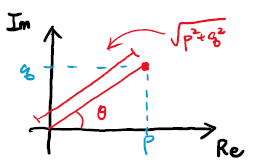
\includegraphics[height=6.5em]{euler}
    \end{minipage}

\end{notation}


%%%%%%%%%%%%%%
\begin{notation}[Side note 2:]
    The \bf{Taylor series expansion} is a polynomial approximation to the any continuous functions $f(x)$,
    for finding the value of $f(k + x)$ given the value of $f(k)$.\\
    
    If the following is a "good" approximation (applicable when $x$ is small enough)
    \aleq{
        f(k+ x) \approx a_0 + a_1 ( x) + a_2 (x)^2 
        + a_3 (x)^3 + ... a_n (x)^n
    }
    with $k$ being a known value, then we can determine $a_0, a_1, ..., a_n$:  
    \aleq{
        a_0 = f(k) \ ,\ 
        a_1 = \eval{\dvv{f(t)}{t}}_{t=k} \ ,\  
        a_2 = \eval{\inv{2!}\dvv[2]{f(t)}{t}}_{t=k} \ ,\ 
        a_3 = \eval{\inv{3!}\dvv[3]{f(t)}{t}}_{t=k} \ ,...
    }
    \aleq{
        \Aboxed{a_n = \eval{\inv{n!}\dvv[n]{f(t)}{t}}_{t=k}}
    }
\end{notation}
\begin{notation}[]
    \begin{proof}
        Let $t=k+x$. Differentiate against $t$ and substitute $x=0$ (so $t$ becomes $k+0=k$),
        \aleq{
            \mat{
                f(k+0) &= &a_0 &+ a_1\cancel{(0)} &+ a_2\cancel{(0)}^2 &+ a_3\cancel{(0)}^3 &+a_4\cancel{(0)}^4 &+...\\[1.2em]
                \eval{\dvv{f(t)}{t}}_{t=k} &= & &+a_1 &+ 2a_2\cancel{(0)} &+ 3a_3\cancel{(0)}^2 &+4a_4\cancel{(0)}^3 &+...\\[1.2em]
                \eval{\dvv[2]{f(t)}{t}}_{t=k} &= & & &+2a_2 &+ (3\cdot 2)a_3\cancel{(0)} &+ (4\cdot 3)a_4 \cancel{(0)}^2 &+...\\[1.2em]
                \eval{\dvv[3]{f(t)}{t}}_{t=k} &= & & & &+ (3\cdot 2)a_3 &+ (4\cdot 3\cdot 2)a_4 \cancel{(0)} &+...
            }
        }
        And so on. 
    \end{proof}

\end{notation}


%%%%%%%%%%%%%%
\subsubsection{Case 3: $b^2-4ac=0$}

This case is problematic in that $\lambda_+ = \lambda_- = \frac{b^2}{2a} \defeq p$.
We can only get 1 independent solution $Ce^{pt}$ by using the $e^{\lambda t}$ trick.

\begin{center}
    \red{
        But mathematicians say if the ODE is of N\Nth order, 
        the general solution must be made of N independent functions.
    }
\end{center}

How to find the remaining independent function in our \nth{2} order ODE? 
The method is called \bf{reduction of order}.

\begin{enumerate}
    \item Let the other independent function be $v(t)e^{pt}$. 
    The goal is to find a suitable $v(t)$ that help it form another solution. 
    First substitute it into the original ODE.
    \aleq{
        a\dvv[2]{t}[v(t)e^{pt}] + b\dvv{t}[v(t)e^{pt}] + c[v(t)e^{pt}] = 0
    }

    \item Do product rule for each term:
    \aleq{
        \dvv[2]{t}[v(t)e^{pt}] &= \dvv[2]{t}v(t)e^{pt} + 2\dvv{t}v(t)\dvv{t}e^{pt}
        + v(t) \dvv[2]{t}e^{pt} \\
        &= e^{pt}\qty[\dvv[2]{t}v(t) + 2p\dvv{t}v(t) + p^2v(t)] \\
        %
        \dvv{t}[v(t)e^{pt}] &= \dvv{t}e^{pt} + v(t)\dvv{t}e^{pt} \\
        &= e^{pt}\qty[\dvv{t}v(t) + pv(t)]
    }

    \item Group terms by derivatives of $v(t)$ and solve it
    \aleq{
        0 &= a\cancel{e^{pt}}\qty[\dvv[2]{t}v(t) + 2p\dvv{t}v(t) + p^2v(t)] 
        + b \cancel{e^{pt}}\qty[\dvv{t}v(t) + pv(t)] + c\qty[v(t)\cancel{e^{pt}}]\\[1.2em]
        %
        &= a\dvv[2]{t}v(t) - 2\cub[red]{(ap+b)}{\substack{=0 \\\text{because }p=\frac{-b}{2a}}} \dvv{t}v(t)
        + \cub[blue]{(ap^2 + bp + c)}{\substack{=0 \\ \text{because }p=\frac{-b}{2a} \text{ is the soln.}\\\text{to } ax^2+bx+c=0}}\\
        %
        &= a\dvv[2]{t}v(t) \\[1.2em]
        %
        v(t) &= C_1t + C_2
    }
\end{enumerate}

where $C_1, C_2$ are some constants. 
Therefore we find the other independent function to be $(C_1t +C_2)e^{pt}$. 
Note that it already contains the first independent function $C e^{pt}$.
We may write 
\aleq{
    \Aboxed{
        f(t) = C_1e^{pt} + C_2 te^{pt} \qquad(\lambda \text{ equal})
    }
}

%%%%%%%%%%%%%%
\begin{notation}[Side note 3:]
    We can use the \bf{Leibniz formula} to compute higher derivatives faster.
    \aleq{
        \dd{(uv)} &= \cus[red]{\dd{u} \cdot v}{1} + \cus[red]{u \dd{v}}{1} \\
        \dd[2]{(uv)} &= \cus[red]{\dd[2]u\cdot v}{1} + \cus[red]{2\dd{u}\cdot\dd{v}}{2} + \cus[red]{u\cdot\dd[2]{v}}{1} \\
        \dd[3]{(uv)} &= \cus[red]{\dd[3]u\cdot v}{1} + \cus[red]{3\dd[2]{u}\cdot\dd{v}}{3} 
            + \cus[red]{3\dd[2]{u}\cdot\dd[2]{v}}{3} + \cus[red]{u\cdot\dd[3]{v}}{1} \\
        &\vdots \\
        \dd[n](uv) &= \sum_{r=0}^{n} C_r^n (\dd[r]{u})(\dd[n-r]{v})
    }
    The coefficients for each term are binomial coefficients $C_r^n = \dfrac{n!}{r!(n-r)!}$, which can be computed beforehand.
\end{notation}


%%%%%%%%%%%%%%
\subsection{Application: Damped Harmonic Oscillator}

Consider a spring-mass system with damping factor on the spring.
When the spring is compressed by a displacement $x$, the forces on it are

\begin{minipage}{0.7\textwidth}
    \begin{itemize}
        \item Spring's elastic force: $-kx$ (Require $k>0$)
        \item Damping force: $-\gamma v$ (Require $\gamma >0$)
    \end{itemize}
\end{minipage}
\begin{minipage}{0.28\textwidth}
    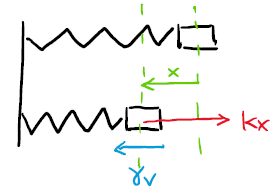
\includegraphics[height=6em]{shm_damp}
\end{minipage}


In a naive model, the damping force is usually assumed proportional and opposite to the mass's velocity.
Otherwise it will be a lot more difficult to calculate.\\

The Newton's \nth{2} Law writes:
\aleq{
    (\text{total force}) = -kx -\gamma v &= ma\\
    m\dvv[2]{t}x(t) + \gamma \dvv{t}x(t) + kx(t) &= 0
}

Substitute $x(t) = Ce^{\lambda t}$, we can find $\lambda_\pm = \dfrac{-\gamma \pm \sqrt{\gamma^2-4mk}}{2m}$.
Then further analyze by the 3 cases 
$\gamma^2-4mk
\begin{cases}
    >0 \\ <0 \\ =0
\end{cases}
$,
which correspond to different physical behaviors.


%%%%%%%%%%%%%%
\subsubsection{Case 1: $\gamma^2-4mk>0$ - Over-damped}

Check the sign of $\lambda_\pm$. Since
\aleq{
    \gamma^2 &> \gamma^2-4mk > 0 \\
    \gamma &> \sqrt{\gamma^2-4mk} \\
    0 &> \frac{-\gamma + \sqrt{\gamma^2-4mk}}{2m} = \lambda_+ \\
}
Also $\lambda_- = \dfrac{-\gamma + \sqrt{\gamma^2-4mk}}{2m} <\lambda_+$. 
So both $\gamma$ are negative. We may write
\aleq{
    x(t) &= C_1 e^{-|\lambda_+|t} + C_2 e^{-|\lambda_-|t} \\
    &= \text{A sum of 2 exponentially decaying functions}
}

\begin{center}
    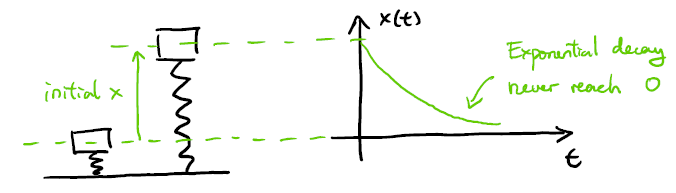
\includegraphics[height=8em]{shm_damp_over}
\end{center}

It is called "over-damped" as the damping force is too large, 
such that the mass can never return to its original position.


%%%%%%%%%%%%%%
\subsubsection{Case 2: $\gamma^2-4mk<0$ - Under-damped}

Write the solution in amplitude form:
\aleq{
    x(t) &= e^{pt} \cdot A\cos{(qt+\phi)} \\
    &= e^{\frac{\gamma}{2m}t} \cdot A\cos\qty(\frac{\sqrt{4mk-\gamma^2}}{2m}t + \phi) \\
    &= (\text{Exponentially Decay})\times(\text{Sinusoidal})
}

\begin{center}
    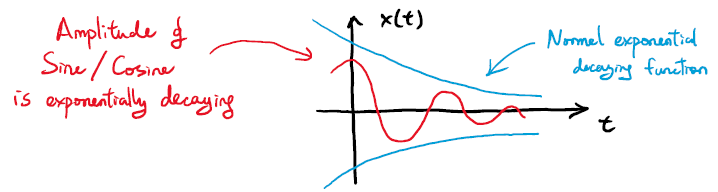
\includegraphics[height=8em]{shm_damp_under}
\end{center}

It is called "under-damped" as the damping force is not strong enough to stop the mass.
The mass will oscillate forever although the amplitude will decrease with time.



%%%%%%%%%%%%%%
\subsubsection{Case 3: $\gamma^2-4mk =0$ - Critical-damped}

The general solution is 
\aleq{
    x(t) = C_1 e^{-\frac{\gamma}{2m}t} + C_2t e^{-\frac{\gamma}{2m}t}
}

\begin{center}
    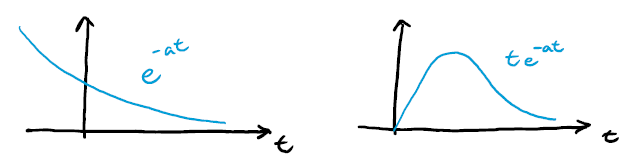
\includegraphics[height=6em]{shm_damp_crit}
\end{center}

It is called "critical-damped" because it is in between the other 2 cases.
It looks like over-damped case but the mass can return to the original position.\\

\linesep
\ul{\bf{Summary in 1 graph}}
\begin{center}
    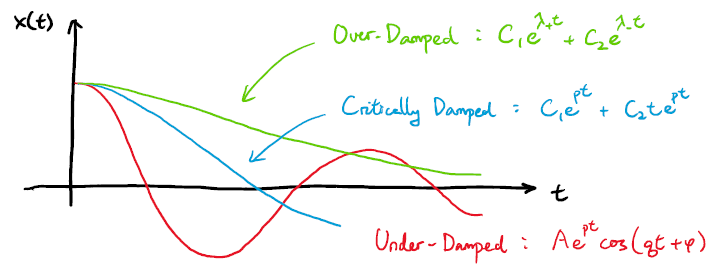
\includegraphics[height=10em]{shm_damp_all}
\end{center}


\linesep
% Section %%%%%%%%%%%%%%%%%%%%%%%%%%%%%%%%%%%%%%%%%%%%%%%%%%%%
\section{Non-homogeneous Constant Coefficient Linear ODE}

Now we consider non-homogeneous linear ODE. For example,
\aleq{
    a\dvv[2]{t}f(t) + b\dvv{t}f(t) + cf(t) = \cus[red]{g(t)}{\substack{\text{non-homogeneous term}\\\text{not containing }f(t)}} \neq 0
}

The general solution to a non-homogeneous linear ODE is made of 2 parts:
\aleq{
    f(t) = f_\blue{c}(t) + f_\red{p}(t)
}
where
\begin{itemize}
    \item $f_\blue{c}(t) =$ \bf{\blue{C}omplementary solution}. 
    It is the general solution to the homogeneous counterpart of the ODE, 
    i.e. the solution to
    \aleq{
        a\dvv[2]{t}f_c(t) + b\dvv{t}f_c(t) + cf_c(t) = 0
    }

    \item $f_\red{p}(t) =$ \bf{\red{P}articular solution}. 
    Its presence is to cancel the non-homogeneous term. 
    \aleq{
        a\dvv[2]{t}f_p(t) + b\dvv{t}f_p(t) + cf_p(t) = g(t)
    }
\end{itemize}

Show by substitution to be clearer:
\aleq{
    g(t) &= a\dvv[2]{t}\qty[f_c(t)+f_p(t)] + b\dvv{t}\qty[f_c(t)+f_p(t)] + c\qty[f_c(t)+f_p(t)] \\[1.2em]
    %
    &= \cub[blue]{\qty[a\dvv[2]{t}f_c(t) + b\dvv{t}f_c(t) + cf_c(t)]}{\substack{\text{Require the parts}\\ \text{constructed by }f_c(t) \\ \text{to become }0}}
    + \cub[red]{\qty[a\dvv[2]{t}f_p(t) + b\dvv{t}f_p(t) + cf_p(t)]}{\substack{\text{Require the parts}\\\text{constructed by }f_p(t) \\ \text{to become }g(t)}} \\[1.2em]
    %
    &= \blue{0} + \red{g(t)}
}

%%%%%%%%%%%%%%
\subsection{An Example of Particular Solution}

Consider a spring-mass system that is subject to gravity. 
The Newton's \nth{2} Law writes:
\aleq{
    m\dvv[2]{t} x(t) = -kx(t) - mg
}

\insertFig{shm gravity}

The simplest way to solve it is by grouping $mg$ into $x(t)$. 
\aleq{
    m\dvv[2]{t} \qty[x(t) + \tkn{mgk}{\cul[blue]{\frac{mg}{k}}}] = -k\qty[x(t) + \frac{mg}{k}]
}\\
\addArrow[blue]{mgk}{(4ex,-4ex)}{$\dfrac{mg}{k}$ is a constant. So $\dvv{t}\qty(\dfrac{mg}{k}) = 0$}
{(0,-3ex)}{(17ex,1ex)}

Then substitute $y(t) = x(t) + \dfrac{mg}{k}$. 
We can see that this ODE of $y(t)$ is the same as equation of motion of a spring-mass system without gravity.
\aleq{
    m\dvv[2]{t} y(t) = -ky(t)
}
which the solution is already known: $y(t) = A\cos\qty(\sqrt{\frac{k}{m}}t+\phi)$.
So we can solve $x(t)$ and identify the particular solution.
\aleq{
    x(t) &= y(t) - \frac{mg}{k} \\
    &= \tkn{shmfc}{\cul[blue]{A\cos\qty(\sqrt{\frac{k}{m}}t+\phi)}} - \tkn{shmfp}{\cul[red]{\frac{mg}{k}}}
}\\[4em]
\addArrow[blue]{shmfc}{(-10ex,-4ex)}{The complementary soln. $f_c(t)$ \\ i.e. the soln. of the homogeneous ODE \\$m\dvv[2]{t} y(t) = -ky(t)$}
{(0,-4ex)}{(-6ex,-4.5ex)}
\addArrow[red]{shmfp}{(10ex,-4ex)}{The particular soln. $f_p(t)$ \\ i.e. for canceling the \\ non-homogeneous term $mg$}
{(0,-2.5ex)}{(1ex,-3.5ex)}


%%%%%%%%%%%%%%
\subsection{Method of Undetermined Coefficients}

Finding a suitable $f_p(t)$ for an arbituary non-homogeneous term $g(t)$ is hard. 
But in most applications, $g(t)$ appears as a combination of common functions.
In these cases, we can make smart guess of what functions is $f_p(t)$ made of.

%%%%%%%%%%%%%%
\subsubsection{Families of common functions \& their derivatives}

Here we consider the function and the constituents of its derivatives as a family.

\begin{itemize}
    \item \ul{Polynomial/Log:} Derivaties of a polynomial must be made of polynomials of lower degree.
    \begin{itemize}
        \item $t^n \to t^{n-1} \to ...\to t^2 \to t \to 1 \quad$ (+ve integral power)
        \item $\ln t \to t^{-1} \to t^{-2} \to ... \quad$ (-ve integral power)
        \item $t^{\half} \to t^{-\half} \to t^{-\frac{3}{2}} \to ...\quad $ (fractional power)
    \end{itemize}

    \item \ul{Trigonometric:} Derivatives of $\sin{(kt)}/\cos{(kt)}$ cycle between themselves.
    \aleq{
        \sin{(kt)} \to \cos{(kt)} \to \sin{(kt)} \to ...
    }
    
    \item \ul{Exponential:} Derivatives of $e^{kt}$ always yield multiples of itself.
    \aleq{
        e^{kt} \to e^{kt} \to e^{kt} \to ...
    }
\end{itemize}

The product between different family yield a set of its own derivatives. For example,
\aleq{
    t^2\sin{t} \to
    \bcase{
        \dd{(t^2\sin{t})} &= 2t\sin{t} + t^2\cos{t} \\
        \dd[2]{(t^2\sin{t})} &= 2\sin{t} + 4t\cos{t} - t^2\sin{t} \\
        \dd[3]{(t^3\sin{t})} &= 6\cos{t} - 6t\sin{t} -t^2\cos{t} \\
        &\vdots
    }
}
One can observe that all its derivatives are made up of 6 different functions,
which form a famaily of function:
\aleq{
    t^2\sin{t} \ , \ t^2\cos{t} \ , \ t\sin{t} \ , \ t\cos{t} \ , \ \sin{t} \ , \ \cos{t}
}

%%%%%%%%%%%%%%
\subsubsection{Method of Undetermined Coefficient}

According to the ODE,
\aleq{
    g(t) &= a\dvv[2]{t}f_p(t) + b\dvv{t}f_p(t) + cf_p(t) \\[1em]
    &= \sum (\text{constant})\cdot(\text{Derivatives of }f_p(t))
}

Conversely, we can make a good guess by \red{assuming $f_p(t) = \dfrac{g(t)}{c} + \qty(\text{Some Derivatives of }g(t))$}. 
Then
\aleq{
    \begin{array}{crcl}
        &\red{c \times \qty[\black{f_p(t)}]}  &= &\red{c \times \qty[\black{\dfrac{g(t)}{c} + \qty(\text{Some Derivatives of }g(t))}]} \\[0.8em]
        &\red{b \times \qty[\black{\dvv{t}f_p(t)}]}  &= &\red{b \times \qty[\black{\dinv{c}\dvv{t}g(t) + \qty(\text{Some Derivatives of }\dvv{t}g(t))}]} \\[0.8em]
        +\Bigr)\  &\red{a \times \qty[\black{\dvv[2]{t}f_p(t)}]}  &= &\red{a \times \qty[\black{\dinv{c}\dvv[2]{t}g(t) + \qty(\text{Some Derivatives of }\dvv[2]{t}g(t))}]} \\[0.8em]
        \hline\\[-1.5em]
        &a\dvv[2]{t}f_p(t) + b\dvv{t}f_p(t) + cf_p(t) &= &g(t) \ \blue{+\ 0}
    \end{array}
}

If we can find a combination of $g(t)$'s derivatives that make up the "(Some Derivatives of $g(t)$)" terms,
such that \blue{all terms on R.H.S except $g(t)$ cancel one another}, 
then we recover $f_p(t)$.


%%%%%%%%%%%%%%
\begin{example}
    \aleq{
        a\dvv[2]{t}f(t) + b\dvv{t}f(t) + cf(t) = t^2+2t
    }

    \begin{itemize}
        \item Sine the ODE is of \nth{2} order, 
        the highest derivative that can be found in "(Some Derivatives of $g(t)$)" is at most $\dvv[2]{t}g(t)$.
        Otherwise it cannot be canceled.

        \item Derivatives of $t^2$ and $t$ both belong to the "integral power polynomial family".

    \end{itemize}

    So we guess 
    \aleq{
        f_p(t) &= (\text{Some combination of }t^2, t, 1) \\
        &= At^2 + Bt + C
    }
    for some constants $A,B,C$ to be solved. 

    \aleq{
        \begin{array}{crcl}
        &\red{c \times \qty[\black{At^2 + Bt + C}]}  &= &\red{c \times \qty[\black{At^2 + Bt + C}]} \\[0.8em]
        &\red{b \times \qty[\black{\dvv{t}(At^2 + Bt + C)}]}  &= &\red{b \times \qty[\black{2At + B}]} \\[0.8em]
        +\Bigr)\  &\red{a \times \qty[\black{\dvv[2]{t}(At^2 + Bt + C)}]}  &= &\red{a \times \qty[\black{2A}]} \\[0.8em]
        \hline\\[-1.5em]
        &a\dvv[2]{t}f_p(t) + b\dvv{t}f_p(t) + cf_p(t) &= & (\red{c}\cdot A)t^2 + (\red{c}\cdot B + \red{b}\cdot 2A)t + (\red{c}\cdot C + \red{b}\cdot B + \red{a}\cdot A) \\
        &g(t) &= & \green{1\times} t^2\ +\ 2t \ \green{+\ 0}
    \end{array}
    }

    By matching coefficients of $t^2, t$ and $1$ respectively, we require
    \aleq{
        \bcase{
            \red{c}\cdot A &= 1 \\
            \red{c}\cdot B + \red{b}\cdot 2A &= 2 \\
            \red{c}\cdot C + \red{b}\cdot B + \red{a}\cdot A &= 0
        }
    }
    which is a system of 3 equations with 3 unknowns $A,B,C$. (Leave the solving to you.)\\

\end{example}

%%%%%%%%%%%%%%
\begin{example}
    \aleq{
        a\dvv[2]{t}f(t) + b\dvv{t}f(t) + cf(t) = \sin{(2t)}
    }

    \begin{itemize}
        \item Sine the ODE is of \nth{2} order, 
        the highest derivative that can be found in "(Some Derivatives of $g(t)$)" is at most $\dvv[2]{t}g(t)$.
        Otherwise it cannot be canceled.

        \item Derivatives of $\sin{2t}$ will cycle between $\sin{2t}$ and $\cos{2t}$. 

    \end{itemize}

    So we guess 
    \aleq{
        f_p(t) &= (\text{Some combination of }\sin{2t}, \cos{2t}) \\
        &= A\sin{2t} + B\cos{2t}
    }
    for some constants $A,B$ to be solved. 

    \aleq{
        \begin{array}{crcl}
        &\red{c \times \qty[\black{A\sin{2t} + B\cos{2t}}]}  &= &\red{c \times \qty[\black{A\sin{2t} + B\cos{2t}}]} \\[0.8em]
        &\red{b \times \qty[\black{\dvv{t}(A\sin{2t} + B\cos{2t})}]}  &= &\red{b \times \qty[\black{2A\cos{2t} - 2B\sin{2t}}]} \\[0.8em]
        +\Bigr)\  &\red{a \times \qty[\black{\dvv[2]{t}(A\sin{2t} + B\cos{2t})}]}  &= &\red{a \times \qty[\black{-4A\sin{2t} - 4B\cos{2t}}]} \\[0.8em]
        \hline\\[-1.5em]
        &a\dvv[2]{t}f_p(t) + b\dvv{t}f_p(t) + cf_p(t) &= & (\red{c}\cdot A - \red{b}\cdot  2B -\red{a}\cdot  4A)\sin{2t} + (\red{c}\cdot  B + \red{b}\cdot  2A - \red{a}\cdot  4B)\cos{2t} \\
        &g(t) &= & \green{1\times}\sin{2t} \ + \ \green{0\times \cos{2t}}
    \end{array}
    }

    By matching coefficients of $\sin{2t}$ and $\cos{2t}$ respectively, we require
    \aleq{
        \bcase{
            \red{c}\cdot A - \red{b}\cdot 2B -\red{a}\cdot 4A &= 1 \\
            \red{c}\cdot B + \red{b}\cdot 2A - \red{a}\cdot 4B &= 0
        }
    }
    which is a system of 2 equations with 2 unknowns $A,B$. (Leave the solving to you.)\\

\end{example}

%%%%%%%%%%%%%%
\begin{example}
    What if particular solution has the same form as the complementary solution?
    \aleq{
        \dvv[2]{t}f(t) - k^2f(t) = e^{k t}
    }

    Its homogeneous counterpart is $\dvv[2]{t}f_c(t) - k^2f_c(t) = 0$. 
    We can immediately write its general solution as 
    \aleq{
        f_c(t) = C_1 e^{kt} + C_2 e^{-kt}
    }

    But the inhomogeneous term $g(t) = e^{kt}$ is also in the same exponential family!
    How do we find a correct $f_p(t)$?
    By \bf{Reduction of order} again.
    
    \begin{enumerate}
        \item Let $f_p(t) = v(t)e^{kt}$.
        The goal is to find a suitable $v(t)$ that helps it form a particular solution that does not belong to the same family as $e^{kt}$. 
        First substitute it into the original ODE and break down by product rule.
        \aleq{
            \dvv[2]{t}[v(t)e^{kt}] - k^2\dvv{t}[v(t)e^{kt}] &= e^{kt} \\
            \dvv[2]{t}v(t)\cdot \ccancel[red]{e^{kt}} + 2\dvv{t}v(t)\cdot k\ccancel[red]{e^{kt}} + \ccancel[blue]{v(t)\cdot k^2e^{kt}} - \ccancel[blue]{k^2v(t)e^{kt}} &= \ccancel[red]{e^{kt}} \\
            \dvv[2]{t}v(t) + 2k\dvv{t}v(t) &= 1
        }

        \item Because this equation has no \nth{0} order of $v(t)$, 
        we can integrate it once to reduce the total order. 
        We arrive at a \nth{1} order inhomogeneous ODE of $v(t)$.
        \aleq{
            \dvv{t}v(t) + 2kv(t) = t + C_3
        }
        where $C_3$ is an arbituary integration constant. 
        Now we have to carry out the standard procedure for solving non-homogeneous equation again:
        \aleq{
            v(t) = v_c(t) + v_p(t)
        }

        \item The complementary solution $v_c(t)$ is trivial:
        \aleq{
            \dvv{t}v_c(t) + 2kv_c(t) &= 0 \\
            v_c(t) &= C_4e^{-2kt}
        }
        with $C_4$ being some constant.

        \item Use method of undetermined coefficients for $v_p(t)$.
        The non-homogeneous term $t+C_3$ is a polynomial of degree 1.
        So its derivative can only be made of $t$ and $1$. 
        Let $v_p(t) = At + B$.
        \aleq{
            \begin{array}{crcl}
            &\red{2k \times \qty[\black{At + B}]}  &= &\red{2k \times \qty[\black{At + B}]} \\[0.8em]
            +\Bigr)\ &\red{1 \times \qty[\black{\dvv{t}(At + B)}]}  &= &\red{1 \times \qty[\black{A}]} \\[0.8em]
            \hline\\[-1.5em]
            &\dvv{t}v_c(t) + 2kv_c(t) &= & (\red{2k}\cdot A)t + (\red{2k}\cdot B + \red{1}\cdot A ) \\
            &g(t) &= & \green{1\times}t \ + \ C_3
        \end{array}
        }

        By matching coefficients of $t$ and $1$ respectively, we require
        \aleq{
            \bcase{
                \red{2k}\cdot A &= 1 \\
                \red{2k}\cdot B + \red{1}\cdot A &= C_3
            }
        }
        which gives $A = \inv{2k}$ and $B = \frac{C_3}{2k}- \inv{4k^2}$.
        So,
        \aleq{
            v_p(t) = \frac{t}{2k} + \qty(\frac{C_3}{2k}- \inv{4k^2})
        }
    \end{enumerate}

    Finally we arrive at 
    \aleq{
        v(t) = v_c(t) + v_p(t) &= C_4e^{-2kt} + \frac{t}{2k} + \qty(\frac{C_3}{2k}- \inv{4k^2}) \\[1em]
        %
        \Rightarrow f_p(t) = v(t)e^{kt} &= C_4e^{-kt} + \qty(\frac{t}{2k})e^{kt}
        + \cub[blue]{\qty(\frac{C_3}{2k}- \inv{4k^2})}{\substack{\text{All are constants.}\\\text{Can combine.}}}e^{kt} \\
        %
        &= \cub[green]{C_4e^{-kt} + C_3'e^{kt}}{\text{Already in }f_c(t)} + \cub[red]{\qty(\frac{t}{2k})e^{kt}}{\text{The true }f_p(t)}
    }

\end{example}

%%%%%%%%%%%%%%
\subsection{Application: Forced Harmonic Oscillator}

Consider a spring-mass system driven by an external force.
When the spring is compressed by a displacement $x$, the forces on it are

\begin{minipage}{0.7\textwidth}
    \begin{itemize}
        \item Spring's elastic force: $-kx$ (Require $k>0$)
        \item Damping force: $-\gamma v$ (Require $\gamma >0$)
        \item External force: $F(t)$ (No restriction)
    \end{itemize}
\end{minipage}
\begin{minipage}{0.28\textwidth}
    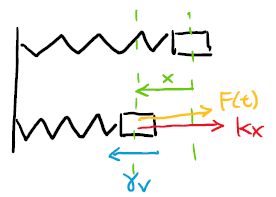
\includegraphics[height=6em]{shm_force}
\end{minipage}

\hfill\\[1em]
The Newton's \nth{2} Law writes:
\aleq{
    (\text{total force}) = -kx -\gamma v + F(t) &= ma\\
    m\dvv[2]{t}x(t) + \gamma \dvv{t}x(t) + kx(t) &= F(t)
}

which is an inhomogeneous \nth{2} order ODE. 
We have already learnt the complementary solution:
\aleq{
    x_c(t) = \begin{cases}
    C_1 e^{\frac{-\gamma + \sqrt{\gamma^2-4mk}}{2m}t} + C_2 e^{\frac{-\gamma - \sqrt{\gamma^2-4mk}}{2m}t} & (\gamma^2-4mk > 0)\\[1em]
    e^{\frac{\gamma}{2m}t} \cdot A\cos\qty(\frac{\sqrt{4mk-\gamma^2}}{2m}t + \phi) & (\gamma^2-4mk <0) \\[1em]
    C_1 e^{-\frac{\gamma}{2m}t} + C_2t e^{-\frac{\gamma}{2m}t} & (\gamma^2-4mk = 0)
    \end{cases}
}

We cannot determine $x_p(t)$ unless we are given the expression of $F(t)$.
One common form of external force is vibration, 
which can be assume as sinusoidal:
\aleq{
    F(t) = F_0 \cos{\omega t}
}

By method of undetermined coefficient, 
we can guess $x_p(t) = A\cos{(\omega t)} + B\sin{(\omega t)}$.
\aleq{
    \begin{array}{crcl}
    &\red{k \times \qty[\black{A\cos{(\omega t)} + B\sin{(\omega t)}}]}  &= &\red{k \times \qty[\black{A\cos{(\omega t)} + B\sin{(\omega t)}}]} \\[0.8em]
    &\red{\gamma \times \qty[\black{\dvv{t}(A\cos{(\omega t)} + B\sin{(\omega t)})}]}  &= &\red{\gamma \times \qty[\black{-\omega A\sin{(\omega t)} + B\omega\cos{(\omega t)}}]} \\[0.8em]
    +\Bigr)\  &\red{m \times \qty[\black{\dvv[2]{t}(-\omega^2 A\cos{(\omega t)} -\omega^2 B\sin{(\omega t)})}]}  &= &\red{k \times \qty[\black{A\cos{(\omega t)} + B\sin{(\omega t)}}]} \\[0.8em]
    \hline\\[-1.5em]
    &m\dvv[2]{t}x_p(t) + \gamma\dvv{t}x_p(t) + kx_p(t) &= & (-\omega^2A m + \omega B \gamma + Ak)\cos{\omega t} \\
        & & & \quad + (-\omega^2Bm -\omega A\gamma +Bk)\sin{\omega t}\\
    &F(t) &= & F_0\cos{2t} \green{\ +\ 0}
\end{array}
}

By matching coefficients of $\cos{\omega t}$ and $\sin{\omega t}$ respectively, we require
\aleq{
    \bcase{
        -\omega^2A m + \omega B \gamma + Ak &= F_0 \\
        -\omega^2B m - \omega A \gamma + Bk &= 0
    }
}
Solving, yield
\aleq{
    A = \frac{F_0(m\omega^2-k)}{(\gamma\omega)^2 + (m\omega^2-k)^2} 
    \quad , \quad 
    B = \frac{F_0\gamma\omega}{(\gamma\omega)^2 + (m\omega^2-k)^2}
}

By combining $\sin/\cos$ into 1 sinusoidal, $x_p(t)$ becomes
\aleq{
    x_p(t) &= A\cos{\omega t} + B\sin{\omega t} \\
    &= \sqrt{A^2+B^2}\cos\qty[\omega t + \tan^{-1}\qty(\frac{B}{A})] \\
    &= \frac{F_0}{\sqrt{(\gamma\omega)^2 + (m\omega^2-k)^2}} \cos\qty[\omega t + \tan^{-1}\qty(\frac{\gamma \omega}{m\omega^2-k})]
}

\hfill\\[1em]
\bf{\ul{Special Case: Resonance}}\\

When the frequency of the external force equals to the natural frequency of harmonic oscillator $\sqrt{\frac{k}{m}}$, 
or $m\omega^2 -k = 0$. 
The displacement $x_p(t)$ becomes
\aleq{
    x_p(t) &= \frac{F_0}{\gamma\omega} \cos\qty[\omega t - \frac{\pi}{2}] \\
    &= \frac{F_0}{\gamma}\sqrt{\frac{m}{k}} \sin{\qty(\sqrt{\frac{k}{m}} t)}
}

In particular, if the damping force also diminish (i.e. $\gamma \to 0$), 
The amplitude of $x_p(t)$ will explode to infinity. 

%%%
\theend
\end{document}